\section{Navigation}\label{sec:navigation}
\subsection{Genutzte Sensoren}\label{subsec:genutzte-sensoren}
Um den Turtlebot durch die Umgebung zu navigieren, braucht es selbstverständlich die Information seiner Sensoren.
Ebenso selbstverständlich sind aber nicht alle Sensoren des Turtlebots gleich für diese Aufgabe geeignet.
So nutzt die Navigation primär zwei Sensoren: Das Lidar des Roboters und sein Odometer, wobei diese für die Erkennung
von ungewöhnlichen Situationen noch von den Reifenkontaktsensoren unterstützt werden.
Sollten die letzteren allerdings auslösen, bleibt dem Algorithmus allerdings leider nichts übrig außer die Bewegung zu
stoppen, um Schaden zu vermeiden und dann das Kartenmaterial neu aufzubereiten, da keine Routine existiert, um herauszufinden,
wie weit der Roboter durch Fremdeinwirkung bewegt wurde.\\


Hätten die zwei Primärsensoren nicht genug information geliefert, hätte auch noch die Option bestanden die Tiefenkamera
des Turtlebots in die Navigation einzubinden, indem man versucht Objekten im Blickfeld der Kamera zu folgen und mithilfe
der Bewegung der Objekte zwischen Bildern festzustellen, wie sich der Roboter bewegt hat.
Da die Primärsensoren aber ausreichende Information liefern war dieser Schritt nicht notwendig, was sowohl algorithmische
als auch Laufzeit Komplexität gespart hat und die Tiefenkamera ist so nur im Einsatz für die Objekterkennung der semantischen
Karte.\\

Die beiden genutzten Sensoren haben hier auch eine Aufgabenteilung: Das Lidar ist primär dafür zuständig, Hindernisse zu
erkennen, während das Odometer die Positionsänderung zwischen Messungen bestimmen soll.
Diese Rollen sind allerdings nicht streng getrennt: Die Messungenauigkeit des Odometers kann mit Information des Lidar
korrigiert werden.
Wenn zum Beispiel das Odometer angibt, dass der Turtlebot $2cm$ nach vorne gefahren ist während das Lidar nur eine
Positionsänderung des Hindernises direkt voraus um $1.9cm$ feststellt, kann der Algorithmus annehmen, dass der Turtlebot
nicht ganz so weit gefahren ist, wie das Odometer angibt.
Das könnte zum Beispiel der Fall sein, wenn die Reifen des Roboters kurz den Grip verlieren und sich so zwar weiterdrehen
aber der Roboter sich nicht wirklich bewegt.
Mithilfe dieser Sensorfusion kann also die relative Position des Roboters bestimmt werden.\\

Hindernisse hingegen werden tatsächlich rein über das Lidar erkannt.
Jeden Augenblick sendet der Roboter Laserpulse aus, mit denen er den Abstand bis zum nächsten Hindernis in diese Richtung
bestimmt.
Hierbei ist noch relevant, dass Teile des Suchfelds des Lidar von der Struktur des Turtlebots geblockt werden und damit
ignoriert werden müssen.
Ansonsten findet das Lidar alle Hindernisse mit Sichtlinie zum Roboter.
Das heißt, dass theoretisch der Roboter in einem leeren Raum eine komplette Karte erstellen könnte, ohne sich zu bewegen,
aber in der Praxis ist fast immer zumindest ein Teil des Raums vom Startpunkt von Hindernissen verdeckt.
\subsection{SLAM Bibliothek}\label{subsec:slam-bibliothek}
Simultaneous Localization and Mapping (SLAM) haben wir nicht selber implementiert, sondern haben hier eine Bibliothek
genutzt.
Natürlich mussten wir hier aber trotzdem Arbeit leisten, um die Bibliothek zu nutzen und in den Rest des Codes zu integrieren.
\subsubsection{turtlebot3\_cartographer} % TODO richtiger Name
Die Bibliothek <lookup name>\cite{navigate_doku} ist eine der standard Bibliotheken der Turtlebot Hersteller.
Sie besteht aus einer Node, die mit dem folgenden Befehl gestartet wird:
\begin{lstlisting}[language=python,label={lst:start_cartographer_node}]
ros2 launch turtlebot3_cartographer cartographer.launch.py
\end{lstlisting}
Das startet die Routine, die das Lidar nutzt, um eine Karte zu erstellen.
Auch gestartet wird eine grafische Oberfläche, die die aktuelle erkundete Karte und die Position des Turtlebot in dieser
anzeigt.
Anfangs ist diese Karte noch größtenteils leer, denn der SLAM Algorithmus braucht zwar nur wenige Informationen um sich
sicher zu sein, dass ein Hindernis existiert aber mehr Informationen braucht um ein Gebiet als frei zu markieren.
Relevant ist auch, dass die Karte nicht auf den Turtlebot zentriert ist, wenn der Turtlebot nahe Hindernissen startet.
Stattdessen wird angenommen, dass diese Hindernisse nahe des Randes des erkundbaren Gebietes, und damit der Karte sind.
Anfangs sieht die Karte wie folgt aus:

\begin{figure}[h!]
    \caption{Eine Karte im direkt nach dem Start des Algorithmus} % TODO
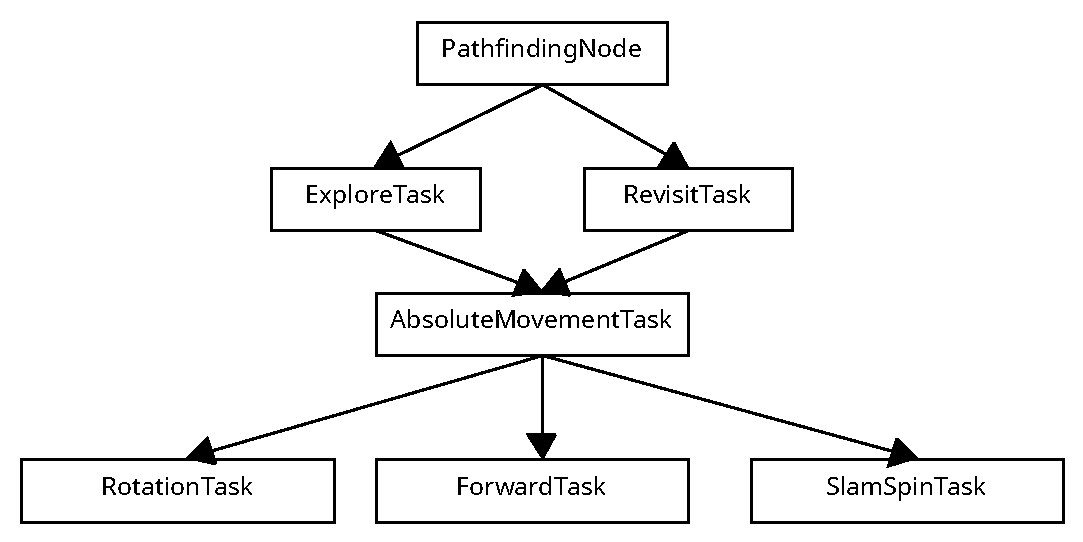
\includegraphics[width=0.8\textwidth]{img/TaskDiagram}\label{fig:map_initial}
\centering
\end{figure}

Besonders ist, dass hier die freien Regionen noch nicht als solche markiert sind, weil der Algorithmus noch nicht genug
Datenpunkte hat.
Sollte man lange genug ohne Bewegung warten startet der Algorithmus sich sicherer zu werden, aber das Kartenmaterial
wird schneller besser, wenn der Turtlebot langsam durch die Umgebung navigiert wird.
Eine fertiggestellte Karte könnte wie folgt aussehen:

\begin{figure}[h!]
    \caption{Eine Karte eines erkundetes Gebietes} % TODO
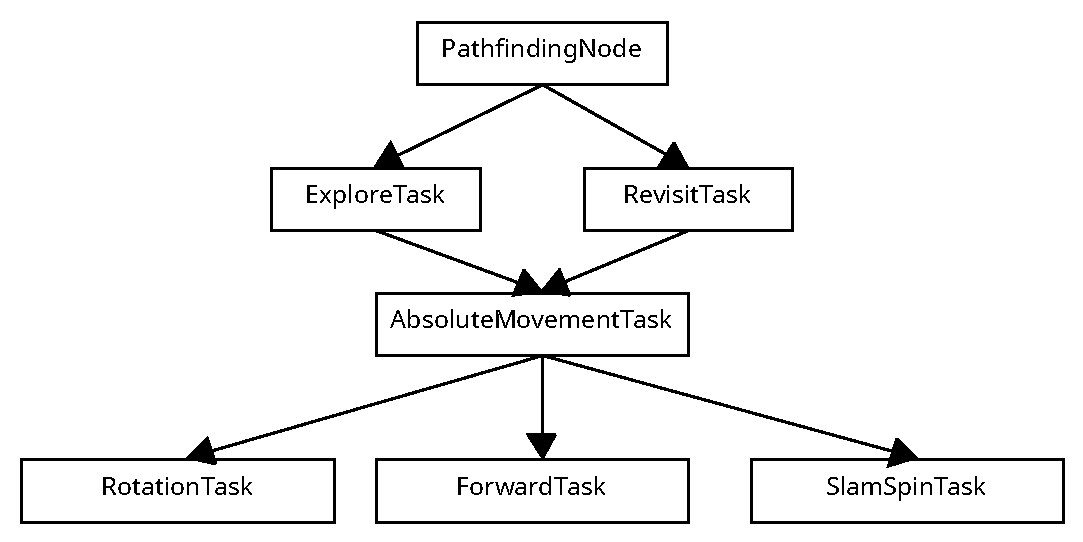
\includegraphics[width=0.8\textwidth]{img/TaskDiagram}\label{fig:map_finished}
\centering
\end{figure}

\subsubsection{Übersetzung zwischen Koordinatensystemen}
Während die Bibliothek zwar ein Koordinatensystem erstellt, ist es leider nicht Deckungsgleich mit dem des Odometers,
dass den Ursprung des Koordinatensystems an anderer Stelle setzt, oder mit dem Koordinatensystem der Navigierung, die zur
Einfachheit der Implementierung den Ursprung in die Ecke der Karte platziert.
Das heißt, dass die Koordinaten die das Odometer angibt in das Koordinatensystem der Navigierung übersetzt werden. \\

Der erste Schritt dabei ist der Transfer von dem Odometer Koordinaten zum SLAM Koordinatensystem.
Dafür gibt die SLAM Bibliothek an, wo sie den Ursprung des Odometer Koordinatensystems wähnt und so kann eine Rotation
und Translation mit jedem Update des Kartenmaterials berechnet werden, welche dann nur noch auf die Koordinaten des
Odometers angewandt werden müssen.
Der zweite Schritt ist dann die statische Rotation und Translation zwischen dem SLAM Koordinatensystem und unserem
Koordinatensystem.
Diese Werte können berechnet werden, da die SLAM Bibliothek auch die Position ihres Ursprungs relativ zur Ecke der Karte
reportiert.\\

Es muss aber nicht nur die Position des Turtlebots zwischen den Systemen transferiert werden.
Auch das Kartenmaterial selber muss von unserem System gelesen und in ein von uns lesbares Format übertragen werden.
Die SLAM Bibliothek gibt die Karte hier im \lstinline{.pgm} Format als zweidimensionale Liste an.
In diesem Format ist diese Liste eine List von Zeilen, was heißt, dass sie zuerst mit der $y$ und dann mit der $x$
Koordinate indiziert werden muss, was uns zunächst nicht aufgefallen ist, was zu vermeidbaren Fehlern geführt hat.\\

Jeder Wert in den inneren Listen stellt dann wiederum ein Quadrat des Bodens da, mit einer größe von $5cm$ in der
Standardkonfiguration.
Dieser Wert rangiert von -1 bis 100, was in der Standardinterpretation eine Intensität eines Grautons repräsentiert und
auch als solche in der grafischen Oberfläche der SLAM Bibliothek genutzt wird, stehen diese Werte in dieser Anwendung
für die Sicherheit, dass an dieser Position ein Hindernis ist.
Dabei steht ein Wert von -1 für eine Position, die der Roboter noch nie gesehen hat und die unsere Navigationssoftware
deshalb als blockiert behandelt, Werte unter 25 sind mit hoher Sicherheit frei und Werte über 65 sind mit hoher Sicherheit
blockiert.
Das lässt den Bereich zwischen 25 und 65 als einen unsicheren Bereich, bei dem sich der SLAM Algorithmus sich noch nicht
sicher ist, ob die Kachel blockiert oder frei ist.
Unser Algorithmus behandelt diese bei der Navigierung, als blockierte Kacheln, um nicht einen Weg durch eine Kachel zu planen,
die dann schließlich doch blockiert ist, sieht diese aber als Ziel für die Navigation um die Unsicherheit zu besiegen.

\subsection{Findung des Navigationsziels}\label{subsec:findung-des-navigationsziels}

\subsubsection{Erkundung}
\subsubsection{Wiederbesuch}
\subsection{Navigieren zum Ziel}\label{subsec:navigierung-zum-ziel}
Nachdem ein Ziel gefunden wurde muss noch der Weg zu diesem Ziel gefunden werden.
Hierfür haben wir den A* Algorithmus eingesetzt, eine Weiterentwicklung des Dijkstra Algorithmus.
\subsubsection{Dijkstra Wegfindung}
Der Dijkstra Algorithmus ist ein Algorithmus um den kürzesten Weg zwischen einem Startknoten und allen anderen Knoten
zu finden, mit der Option früher abzubrechen, wenn der Weg zu einem bestimmten Endknoten gefunden ist.
Dabei ist er ein greedy Algorithmus der schrittweise den kürzesten Weg von dem Startknoten ausgehend bestimmt.
Die einzigen Limitierungen an den Graphen, die der Dijkstra Algorithmus stellt, sind, dass der Graph verbunden sein muss
(sonst existieren einige Wege nicht) und dass keine Gewichtung einer Verbindung negativ sind.
Eine negative Gewichtung kann dazu führen, dass der Algorithmus nicht den optimalen Weg zum Endknoten findet, weil der Algorithmus abbricht, bevor der negative
Weg in Betrachtung gezogen wird.\\

Der erste Anspruch kann in unserem Problem nicht garantiert werden - es ist durchaus möglich, dass Teile des sichtbaren
Gebietes nicht erreichbar sind, weil der Weg dahin zu dünn für den Turtlebot ist.
Manche Zielpunkte sind also nicht navigierbar, was wir bei der Implementierung beachten werden müssen.\\

Die zweite Bedingung können wir hingegen garantieren, weil die Gewichtungen unseres Graphen der Entfernung zwischen
zwei Knoten entsprechen und damit nicht negativ sein können.
Das die Realität des Systems negative Gewichte verbietet ist durchaus üblich, was diese Bedingung des Dijkstra Algorithmus
in der Praxis selten relevant macht.\\



Der Algorithmus selber besteht aus vier Schritten: Initialisierung, Wahl des nächsten Knotens, Verarbeitung des Knotens und Wegrückverfolgung,
wobei die mittleren beiden Schritte wiederholt werden, bis der Algorithmus fertig ist.

In der Initialisierung wird die Distanz bis zum Startknoten auf 0 gesetzt und die Entfernung zu allen anderen Knoten auf
$\infty$ gesetzt.
Ebenfalls werden alle Knoten als unbesucht markiert.\\

Dann wird der nächste Knoten gewählt.
Dieser ist der Knoten mit der kleinsten Distanz, der noch nicht besucht wurde.
Dieser lässt sich trivial in $O(n)$ Laufzeit finden, indem alle Knoten geprüft werden, aber mithilfe von Datenstrukturen
wie Priority Queues lässt sich das auf $O(\log n)$ reduzieren.\\

Als letzter Schritt vor der Wiederholung kommt dann die Verarbeitung des Knotens.
Hierbei wird für jeden Nachbarn des ausgesuchten Knotens geprüft, ob die Distanz des ausgesuchten Knotens zusammen mit der
Gewichtung der Verbindung zwischen den beiden Knoten kleiner ist als die aktuelle Distanz des Nachbarn.
Wenn ja, wird die Distanz des Nachbars dann auf diesen Wert gesetzt und der aktuelle Knoten im Nachbarn als Vorgänger
eingetragen.
Wenn dieser Schritt abgeschlossen ist, wird der aktuelle Knoten dann noch als besucht markiert.\\

Nachdem alle Knoten verarbeitet wurden (oder der Endknoten verarbeitet wurde, wenn nur ein Ziel existiert) kann dann eine
Route gefunden werden.
Dafür wird ein Zielknoten gewählt und von diesem dann der Kette von Vorgängerknoten gefolgt, bis diese den Startknoten
erreicht.
Diese Kette kann dann invertiert werden, um die Route zum Ziel zu erhalten.\\
\subsubsection{A* Heuristik}\label{subsubsec:astar}
Während der Dijkstra Algorithmus den schnellsten Weg zu allen Knoten findet, findet der A* Star Algorithmus nur den
schnellsten Weg zu einem bestimmten Zielknoten.
Dafür ist der Algorithmus aber performanter, da er Knoten primär in der Richtung des Zielknotens untersucht mithilfe
einer Heuristik.\\

Um diese Richtung festzustellen, nutzt der Algorithmus eine Heuristik.
Diese muss die Entfernung zwischen zwei beliebigen Knoten angeben und, damit A* tatsächlich die kürzeste Entfernung
findet, muss diese Heuristik die Entfernung unterschätzen.
Wenn dies nicht der Fall ist, findet A* zwar immer noch einen Weg, dieser ist aber nicht mehr garantiert der Kürzeste.\\

Der einzige Unterschied im Algorithmus zu Dijkstra ist, wie der nächste Knoten ausgewählt wird: Auch A* betrachtet nur
Knoten, die noch nicht besucht wurden, nimmt aber nicht den Knoten mit der niedrigsten Distanz, sondern den Knoten mit der
niedrigsten Summe aus Distanz und Heuristik bis zum Ziel.
So werden Knoten bevorzugt, die näher am Zielknoten liegen.\\

Sollte man sowohl Dijkstra als auch A* auf einer 2D-Ebene ausführen, lässt sich der Vorteil einfach visualisieren:
Dijkstra besucht Punkte in einem Kreis um den Startpunkt bis der Kreis den Endpunkt beinhaltet während die besuchten Punkte
von Dijkstra eine Ellipse bilden, die, wenn der Algorithmus beendet ist den Start und Endpunkt als Brennpunkte hat.\\

\begin{figure}[h!]
    \caption{Ein Vergleich zwischen dem Suchverhalten des Dijkstra und Astar Algorithmus} % TODO
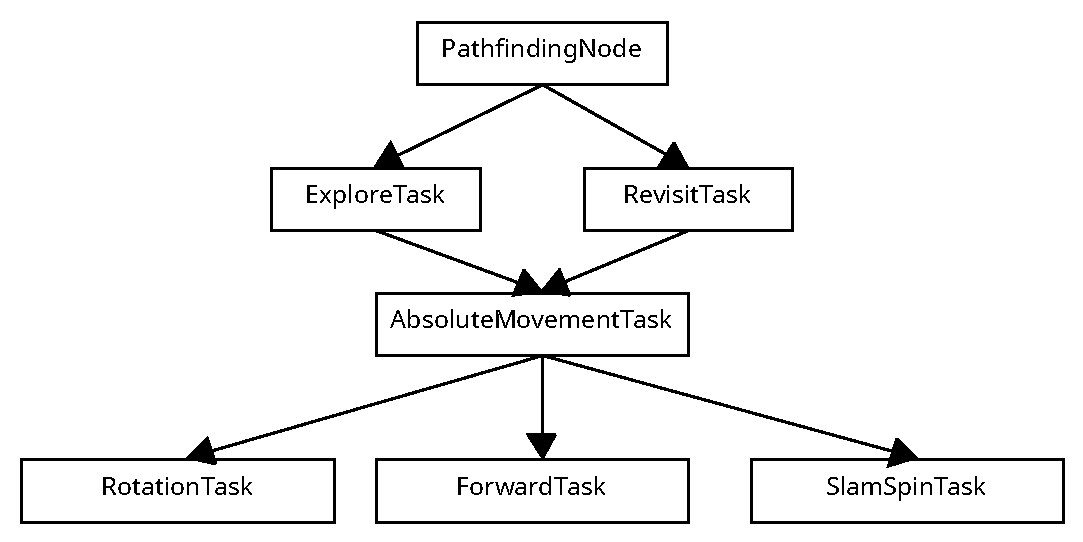
\includegraphics[width=0.8\textwidth]{img/TaskDiagram}\label{fig:dijkstra_v_astar}
\centering
\end{figure}

Solange nur der Weg zu einem Knoten interessant ist, bietet A* gegenüber Dijkstra also eine bessere Performance.
Da unser Anwendungsfall ist, zu einem bestimmten Punkt zu navigieren, ist das bei uns der Fall.
Es gibt dennoch einen Aspekt des Problems, der zu wiederholter Ausführung des A* Algorithmus führen könnte, der womöglich
Dijkstra performanter machen könnte: Es ist möglich, dass der Turtlebot einen Ort durch einen Spalt gesehen hat, durch
den er nicht durchfahren kann und somit unmöglich Endpunkte probiert werden.
Jeder dieser Endpunkte erzeugt eine eigene A* Rechnung, auch wenn sie sich eine Dijkstra Rechnung teilen könnten.
Sollte dies in der Praxis ein Laufzeitproblem erstellen besteht hier die Option die Distanzen des A* Algorithmus mit
einer neuen Heuristik für einen neuen Endpunkt wiederzuverwenden, da sich die Distanzen vom Startpunkt nicht mit
verschiedenen Endpunkten ändern, nur die Reihenfolge in der die Knoten ausgewertet werden.
Dieser Ansatz ist aber komplizierter in der Implementierung und war für unsere Performancebedürfnisse nicht notwendig und
wurde daher von uns nicht implementiert.
\subsubsection{Implementierung}
Unsere Implementierung in Python besteht aus einer Methode, die Bewegungsaufgaben[\ref{subsubsec:taskmanagement}] erzeugt
und einer Hilfsklasse, die den Algorithmus implementiert.
Hier haben wir die Implementierung in drei Teile unterteilt: Das Erstellen des Graphen, die Anwendung des A* Algorithmus
und die Extraktion der Route.\\

Der erste Aspekt, die Erstellung des Graphen wird in der Initialisierung der AstarMap Hilfsklasse durchgeführt.
Diese verlangt die AreaMap die bei der Positionsfindung erzeugt wurde und die aktuelle Position.
Mit diesen Informationen erstellt sie dann eine 2D Liste in der aus jeder Node er AreaMap eine Node der AstarMap erstellt
wird.
Auch wird eine Priority Queue für die Nodes erstellt, in der die noch nicht besuchten, aber bereits bekannten, Nodes gelistet
werden und es wird die Node der aktuellen Position mit der Distanz 0 hinzugefügt.
Das weicht von der Referenzimplementation ab, wird aber näher bei dem Fragment für die $astar\_run$ Methode erklärt.
\begin{lstlisting}[language=python,label={lst:astar_map_init}]
def __init__(self, area_map, pos, logger, heuristic=manhatten_distance):
self.logger = logger
self.heuristic = heuristic
self.priority_queue = PriorityQueue()
self.nodes_2d: List[List[AstarNode]] = []
for y, row in enumerate(area_map):
    self.nodes_2d.append([])
    for x, node in enumerate(row):
        astar_node = AstarNode(node, area_map, self)
        self.nodes_2d[y].append(astar_node)

pos_node = self.nodes_2d[int(pos.y)][int(pos.x)]
pos_node.score = 0
self.priority_queue.put((0, pos_node))
for node in (n for row in self.nodes_2d for n in row):
    node.post_init()
\end{lstlisting}

Die referenzierte $post\_init$ Methode der AstarNode ist simple und registriert nur die Nachbarn der Node aus der
unterliegenden AreaMap, die in der Postions findung erstellt wurde.
Diese Methode kann nicht in die $\_\_init\_\_$ Methode der AstarNode integriert werden, da Nachbarschaft symmetrisch ist
und so beide Nachbarn vor dem jeweils anderen erstellt werden müssten, was natürlich unmöglich ist.
So werden zuerst alle Nodes erstellt und danach die Verbindungen zwischen den Nodes initialisiert.
\begin{lstlisting}[language=python,label={lst:astar_node_init}]
def post_init(self):
    self.neighbors = [self.astar_map.nodes_2d[neighbor.y][neighbor.x]
                        for neighbor in self.node.neighbors]
\end{lstlisting}

Kommen wir jetzt zum Kernstück des A* Algorithmus, der $run\_astar$ Methode.
Sie beginnt damit, sich den Zielknoten zu merken und beginnt dann eine Schleife, die zwei Austrittsmöglichkeiten hat;
Es sind keine Knoten in der Priority Queue mehr oder die aktuelle Node ist die Target Node, die der Algorithmus sich gemerkt
hat.
In dem ersten Scenario bricht die Methode mit einer Fehlermeldung ab, weil sie keinen Weg finden könnte, während im
zweiten Scenario der Algorithmus den kürzesten Weg zum Ziel gefunden hat.
In jedem Durchlauf der Schleife wird dann der Knoten mit dem kleinsten Wert aus der Priority Queue entfernt.
Für jeden befahrbaren Nachbarn wird dann geprüft, ob der Weg über die aktuelle Node schneller ist.
Wenn ja, wird die Node in der Priority Queue mit dem neuen Wert aktualisiert oder der Queue hinzugefügt, falls sie
zum ersten Mal gesehen wurde.
Das ist equivalent zu der Methode zu vermerken, welche Knoten bereits besucht wurden, da wenn ein Knoten evaluiert wird
hat er die niedrigstmögliche Distanz da der Graph überall die Gewichtung 1 hat und somit die Distanz der evaluierten
Knoten monoton steigt.
Auch ist die Inklusion mit aller Knoten mit $\infty$ Distanz equivalent zu ihrer Inklusion erst, wenn ein Nachbar evaluiert wird.
In dem Standardalgorithmus werden diese Knoten auch erst relevant, wenn eine andere Distanz für diese gesetzt wird, was
dieselbe Bedingung wie für die Inklusion in die Priority Queue ist.
\begin{lstlisting}[language=python,label={lst:run_astar}]
target = self.nodes_2d[int(target.y)][int(target.x)]
while not len(self.priority_queue) == 0:
    node_score, node = self.priority_queue.pop()
    if node == target:
        self.logger.info('Finished the path to target')
        return node
    for neighbor in node.neighbors:
        if (neighbor.obstructed or
            not (0 <= node.node.obstruction < free_threshold)):
            continue
        neighbor_score_via_current = node_score + 1 + self.heuristic(neighbor, target)
        if neighbor_score_via_current < neighbor.score:
            neighbor.predecessor = node
            neighbor.score = neighbor_score_via_current
            updated = self.priority_queue.update_elem(
                neighbor, (neighbor_score_via_current, neighbor)
            )
            if not updated:
                self.priority_queue.put((neighbor_score_via_current, neighbor))
raise ImpossibleRouteException(f"No Route to {target} found")
\end{lstlisting}

Nachdem diese Methode durchgelaufen ist, ist die schnellste route zu dem Zielknoten definiert, aber was für die weitere
Bewegungsplanung interessant ist, ist der nächste Knoten, zu dem der Roboter fahren muss.
Dafür startet die Bewegungsplanungsmethode mit dem Zielknoten und geht entlang der Vorgängerknoten und registriert alle
Knoten in eine Liste bis der Startknoten erreicht wird.
Der zweite Knoten in der Liste (der erste ist der Startknoten) ist dann der nächste Knoten der angefahren werden muss.

\begin{lstlisting}[language=python,label={lst:pathfinding}]
current_node = end_node
path = []
while current_node.predecessor is not None:
    path = [current_node] + path
    current_node = current_node.predecessor
self.task_list = [SlamSpinTask(self.pathfinding),
                  ForwardTask(self.pathfinding, path[1].node),
                  RotationTask(self.pathfinding, path[1].node)]
\end{lstlisting}
\subsubsection{Verwaltung der aktuellen Aufgabe} \label{subsubsec:taskmanagement}
Wie am Ende der letzten Sektion vielleicht schon ersichtlich wird, werden in unserem Projekt Bewegungen als einzelne
Aufgaben dargestellt.
Diese bestehen meist aus anderen, spezifischeren Aufgaben wie in dem folgenden Abhängigkeitsdiagramm dargestellt.
\begin{figure}[h]
    \caption{Ein Diagramm der Abhängigkeiten zwischen Tasks}
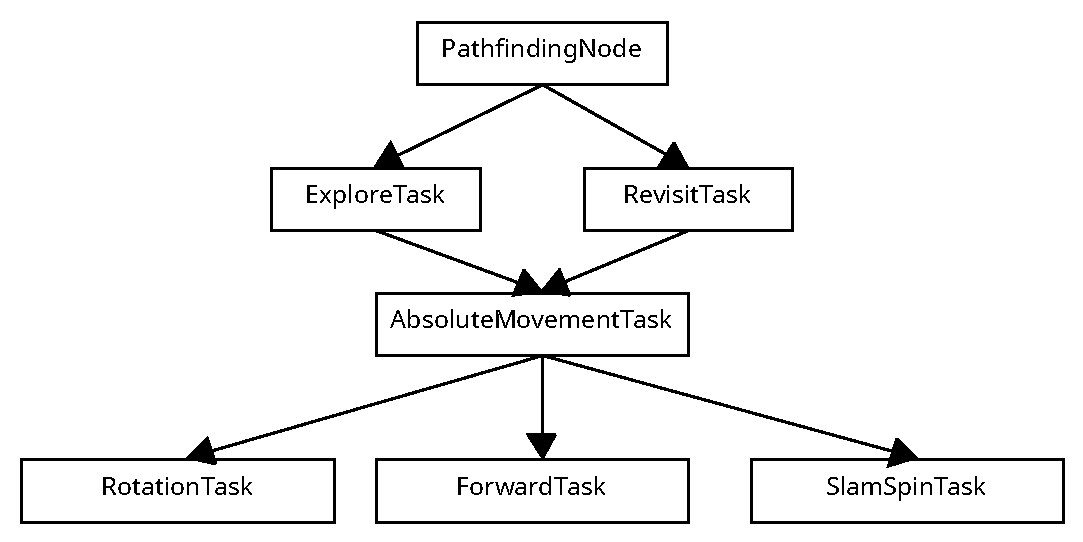
\includegraphics[width=0.8\textwidth]{img/TaskDiagram}\label{fig:taskdiagram}
\centering
\end{figure}
Die Hierarchie beginnt mit der PathfindingNode, die eine List von Aufgaben registriert hat und alle $0.1s$ prüft, ob die
aktuelle Aufgabe fertiggestellt ist (und diese aus der Liste entfernt, wenn das der Fall ist) und dann die aktuelle
Aufgabe ausführt.\\

Auf dieser Ebene ist die Aufgabe eine Erkundungsstrategie, entweder ExploreTask mit der eine noch unbekannte Umgebung
erkundet wird oder RevisitTask der aktiviert wird, wenn ExploreTask keine neuen Gebiete mehr sieht und zu dem Punkt
navigiert, der am längsten nicht besucht wurde.
Dafür finden sie bei ihrer Initialisierung ein passendes Ziel und erstellen einen AbsoluteMovementTask zu diesem Ziel,
an den sie alle weitere Ausführung delegieren und mit dessen Fertigstellung sie sich selber als fertig markieren.\\

Dieser wiederum führt eine A* Wegfindung[\ref{subsubsec:astar}] während seiner Initialisierung durch und erstellt dabei
drei weitere Aufgaben, die dann nacheinander abgearbeitet werden bis sie abgeschlossen sind: Ein RotationTask,
ein ForwardTask und ein SlamSpinTask.
Diese beschreiben wiederum eine konkrete Bewegung mit einem Zielzustand, dessen Erreichung die Aufgabe als fertig markiert.\\

RotationTask beginnt damit, die Richtung zu der Zielposition zu ermitteln und dann die Differenz zwischen dieser und der
aktuellen Ausrichtung festzustellen.
Nachdem diese bekannt ist, beginnt er eine Drehung und prüft die Ausrichtung des Turtlebots durchgehend bis die
Zielausrichtung erreicht ist.
Wenn die Zielausrichtung erreicht ist, sendet dieser Task dann noch das Stop-Signal und markiert sich als fertig.\\

Darauf folgt der ForwardTask, der eine Vorwärtsbewegung startet.
Dabei nimmt er an, dass ein vorhergehender RotationTask bereits die Ausrichtung angepasst hat und wartet, bis die
aktuelle Position des Turtlebots den Zielknoten erreicht, woraufhin auch diese Aufgabe ein Stop-Signal sendet und sich
als fertig markiert.\\

Die letzte Aufgabe, SlamSpinTask, unterscheidet sich dadurch, dass sie nicht von einem Zielknoten abhängig ist.
Statt näher an das Ziel zu kommen, ist die Aufgabe des SlamSpinTask Daten für die Kartografierung zu liefern.
Dafür wird der Turtlebot einen Moment rotiert, was zwar die allgemeine Bewegung durch die ``Verschwendung'' von Zeit
verlangsamt, aber ideal dafür ist, die Konfidenz des Kartografierungsalgorithmus zu erhöhen, indem mehr Sensordaten ohne
Bewegung geliefert werden.
Dadurch wird zukünftige Navigation besser, da das Kartenmaterial verbessert wurde.

